\chapter{WORK COMPLETED}
\section{Outcome/Lesson Learnt}
\subsection{HomePage}
A home page is the default or front page of a site. It is the first page that visitors see when they load a URL. Web managers can control the home page as a way of directing the user experience.
\begin{figure}[h]
    \centering
    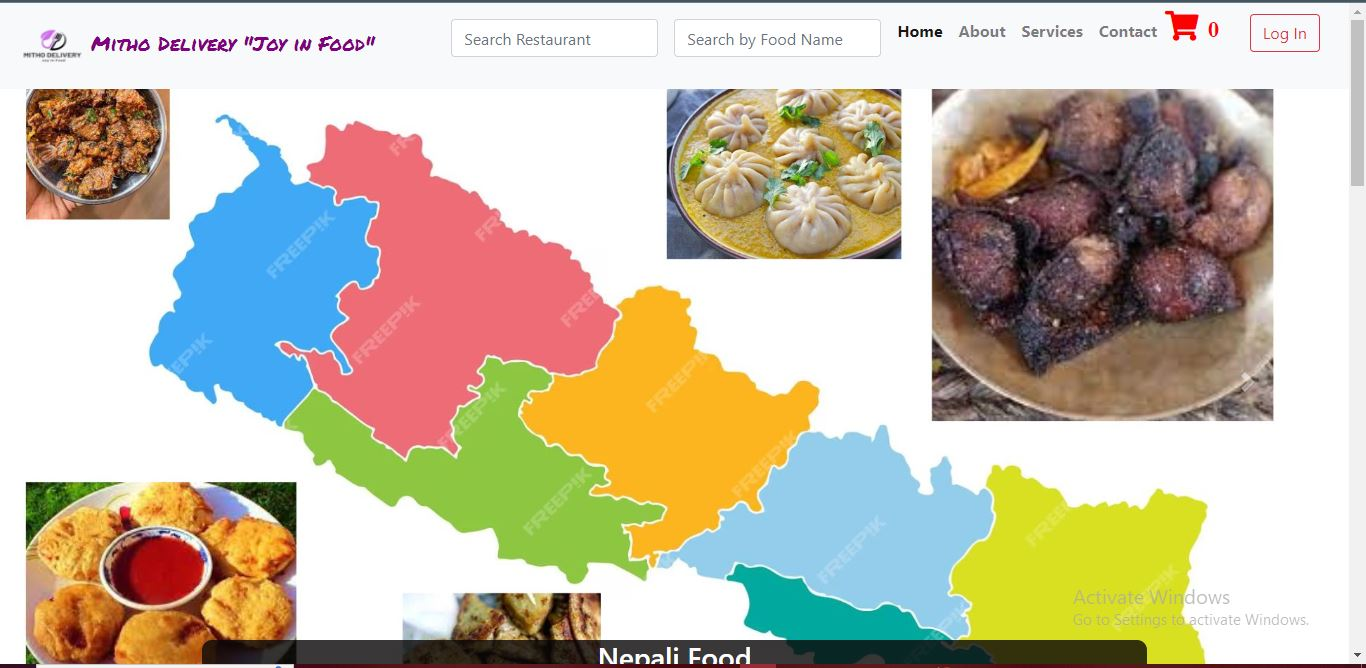
\includegraphics[height=7cm]{img/Graphics/home ui.JPG}
    \caption{HomePage}
\end{figure}

\subsection{About Us}
An "About Us" page on a website provides information about the site which includes details about the website's mission, team members. This page helps build trust and transparency with website visitors.
\begin{figure}[h]
    \centering
    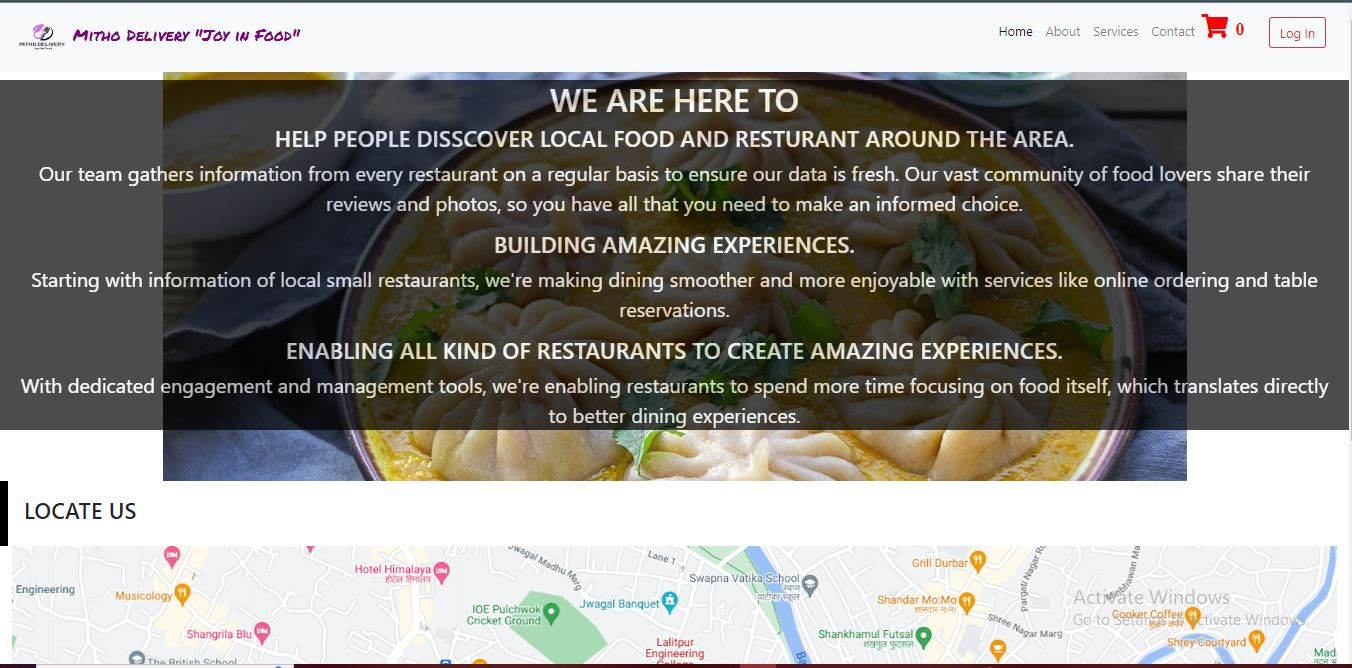
\includegraphics[height=6cm]{img/Graphics/about ui.JPG}
    \caption{About Us}
\end{figure}

\subsection{Services}
A "Services" page on a website is where the organization or business describes the products or services it offers.
\begin{figure}[h]
    \centering
    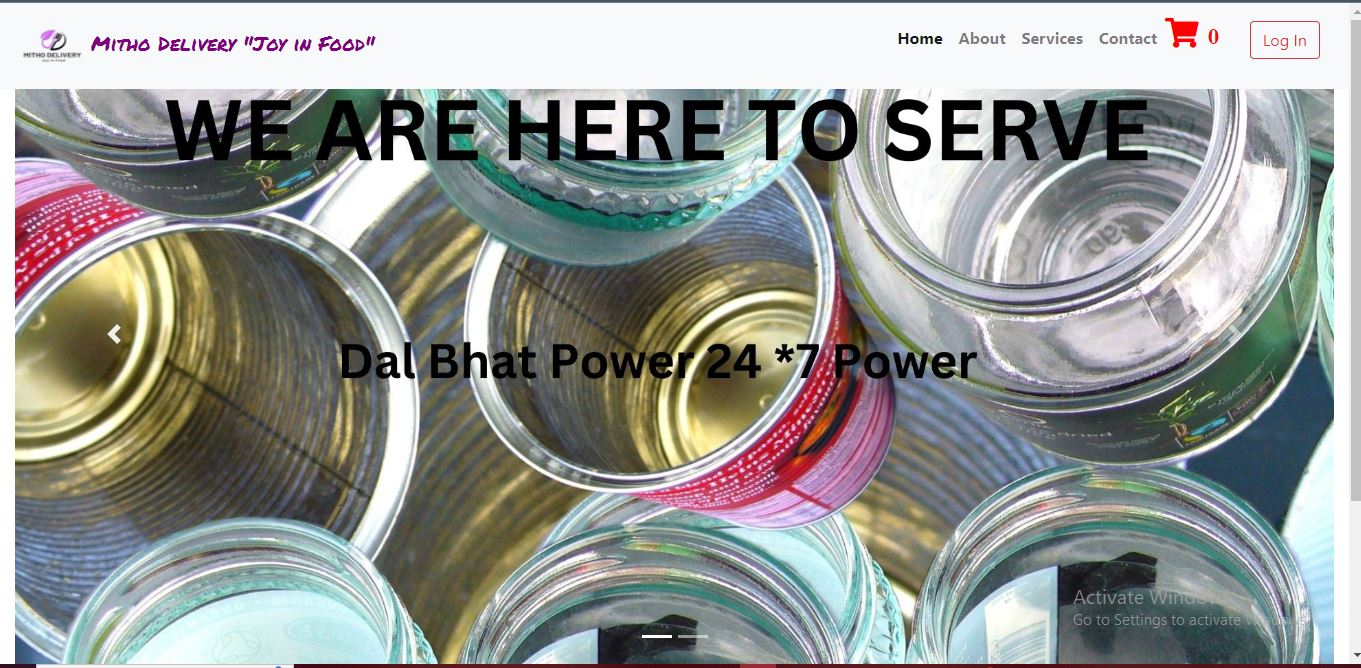
\includegraphics[height=7cm]{img/Graphics/service.JPG}
    \caption{Services}
\end{figure}

\subsection{Contact}
The "Contact" page on a website is a crucial section that enables visitors to get in touch with the website owner or organization. It typically includes information and tools for communication
\begin{figure}[h]
    \centering
    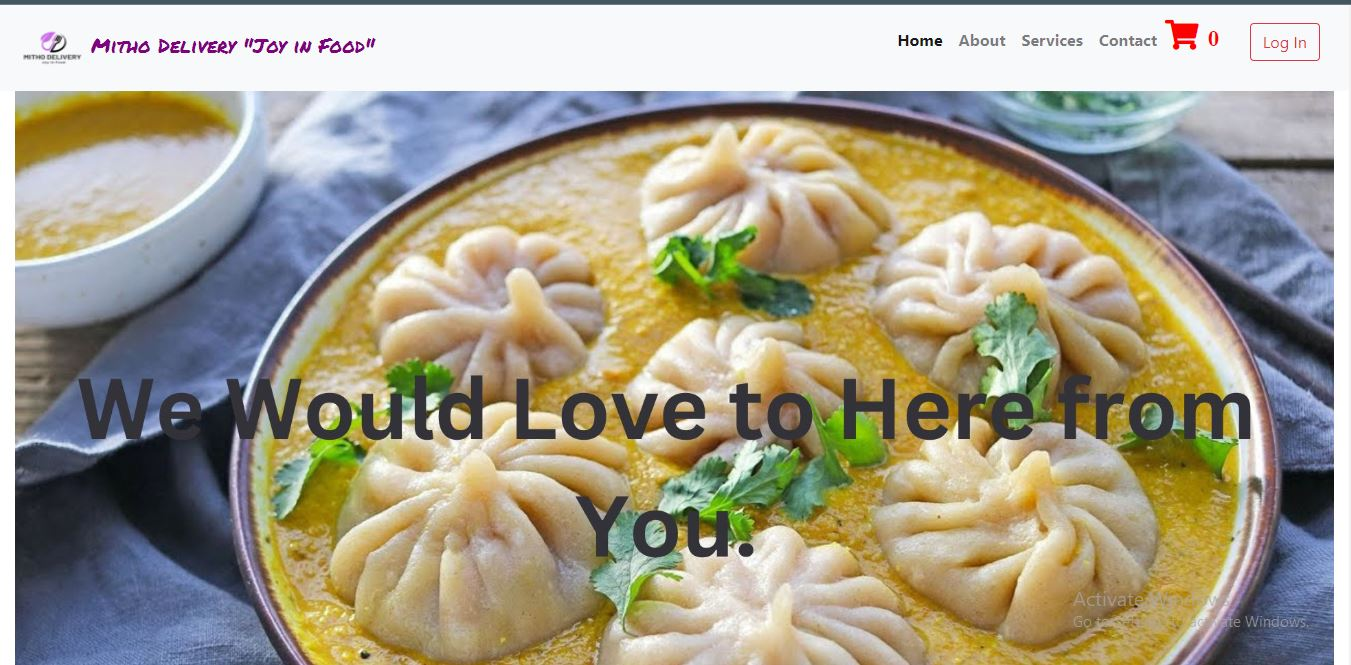
\includegraphics[height=7cm]{img/Graphics/contact.JPG}
    \caption{Contact}
\end{figure}

\newpage
\subsection{Cart}
A "Cart" on a website is a virtual shopping cart or basket that allows users to collect and store items they want to purchase while browsing the site. 
\begin{figure}[h]
    \centering
    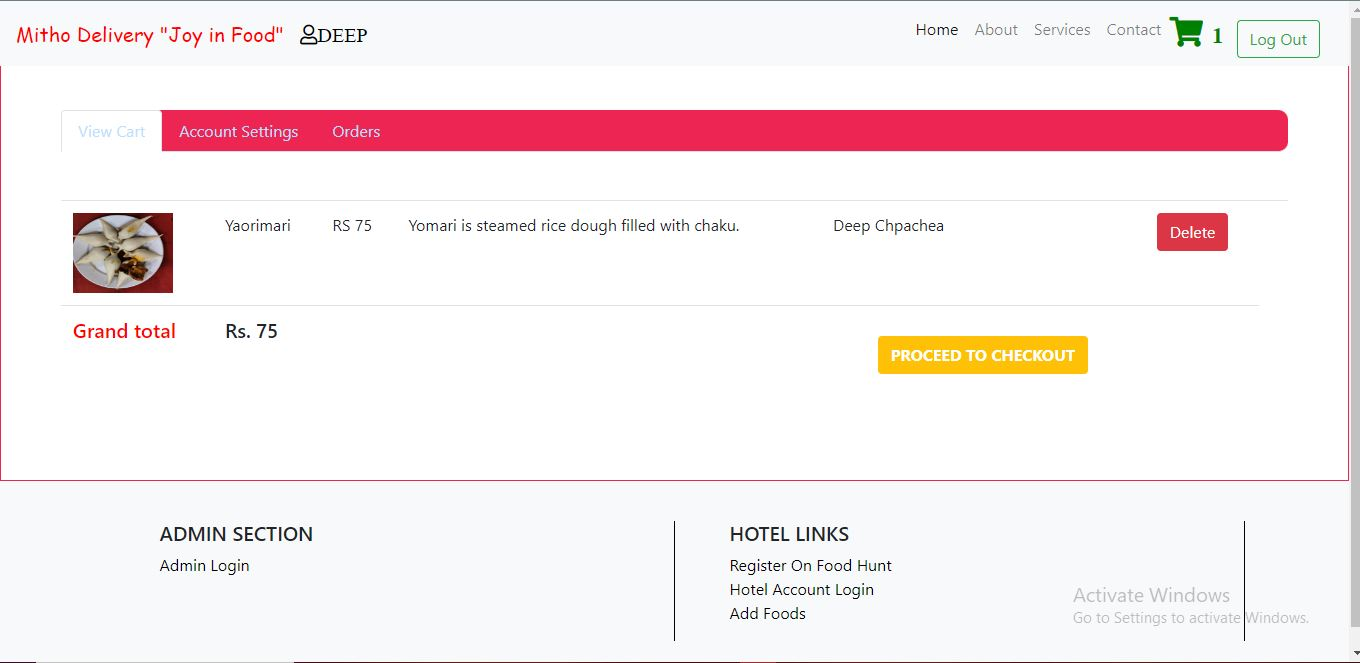
\includegraphics[height=7cm]{img/Graphics/cart ui.JPG}
    \caption{Cart}
\end{figure}

\subsection{Food Details}
A Food Details page on a website offers in-depth information about a specific food item. This page helps users make informed decisions about the food they are interested in.
\begin{figure}[h]
    \centering
    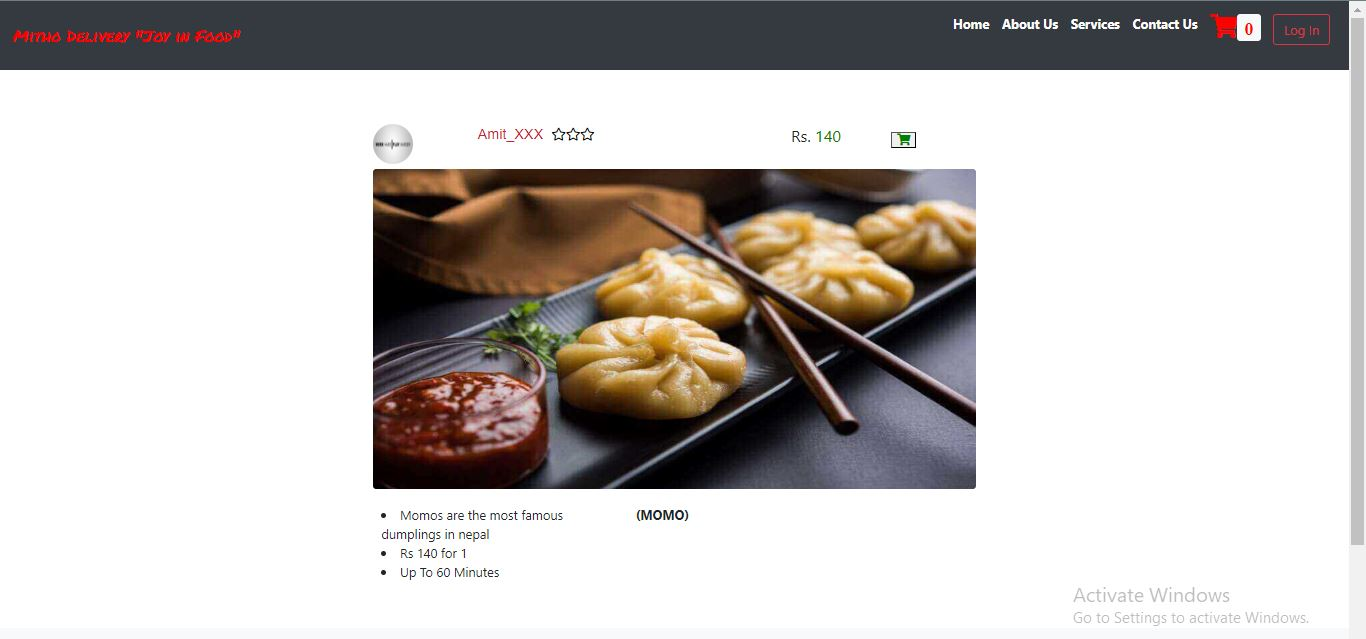
\includegraphics[height=7cm]{img/Graphics/food detail ui.JPG}
    \caption{Food Details}
\end{figure}

\newpage
\subsection{Restuarant Details}
A restaurant detail page on a website is a dedicated section that offers comprehensive information about a specific restaurant. This page is typically designed to help potential customers learn more about the restaurant's offerings, location, and other essential details. 
\begin{figure}[h]
    \centering
    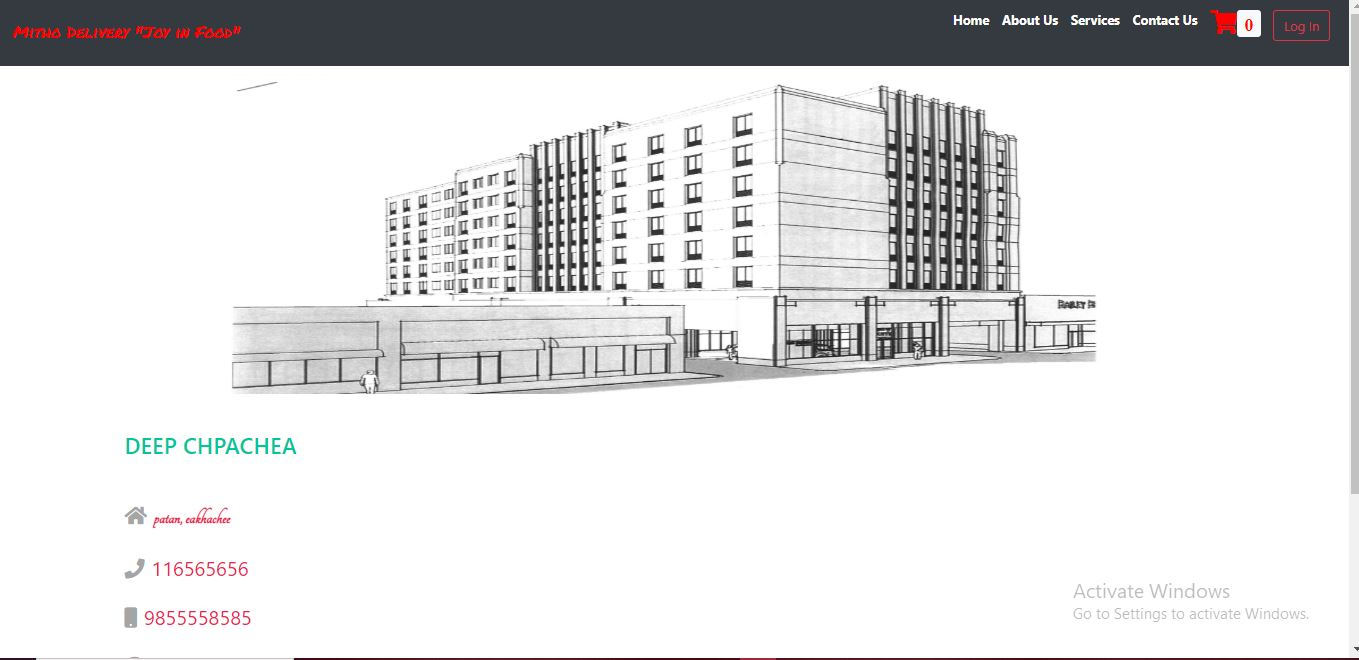
\includegraphics[height=7cm]{img/Graphics/hotel detail ui.JPG}
    \caption{Restuarant Details}
\end{figure}

\subsection{Search Bar}
A search bar on a food ordering website is a critical feature that allows users to quickly find specific dishes or restaurants within the platform. 
\begin{figure}[h]
    \centering
    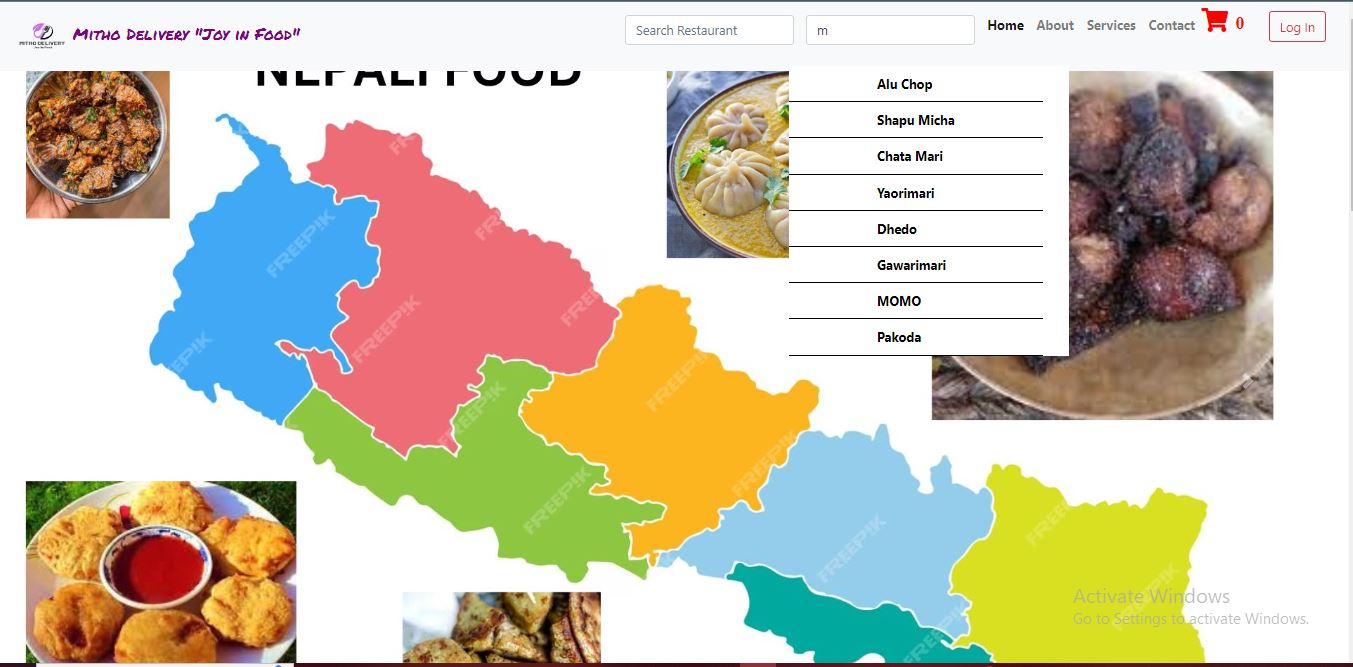
\includegraphics[height=7cm]{img/Graphics/search bar ui.JPG}
    \caption{Search Bar}
\end{figure}

\newpage
\subsection{Login}
The act of logging in verifies the user's identity, granting them authorized access to restricted resources or functionalities within the system.
\begin{figure}[h]
    \centering
    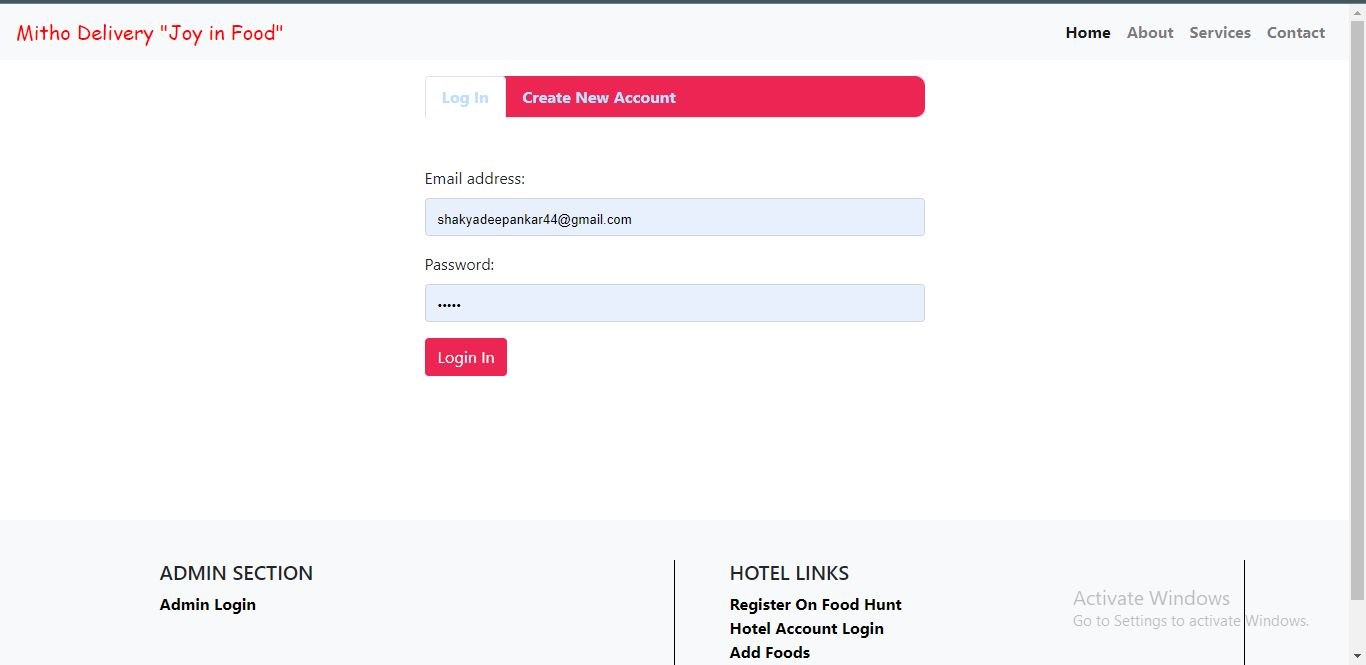
\includegraphics[height=7cm]{img/Graphics/login ui.JPG}
    \caption{Login}
\end{figure}

\subsection{Restuarant Signup}
Signup, also known as registration, refers to the process through which a restuarant creates a new account or profile on a digital platform, such as a website, app, or service. 
\begin{figure}[h]
    \centering
    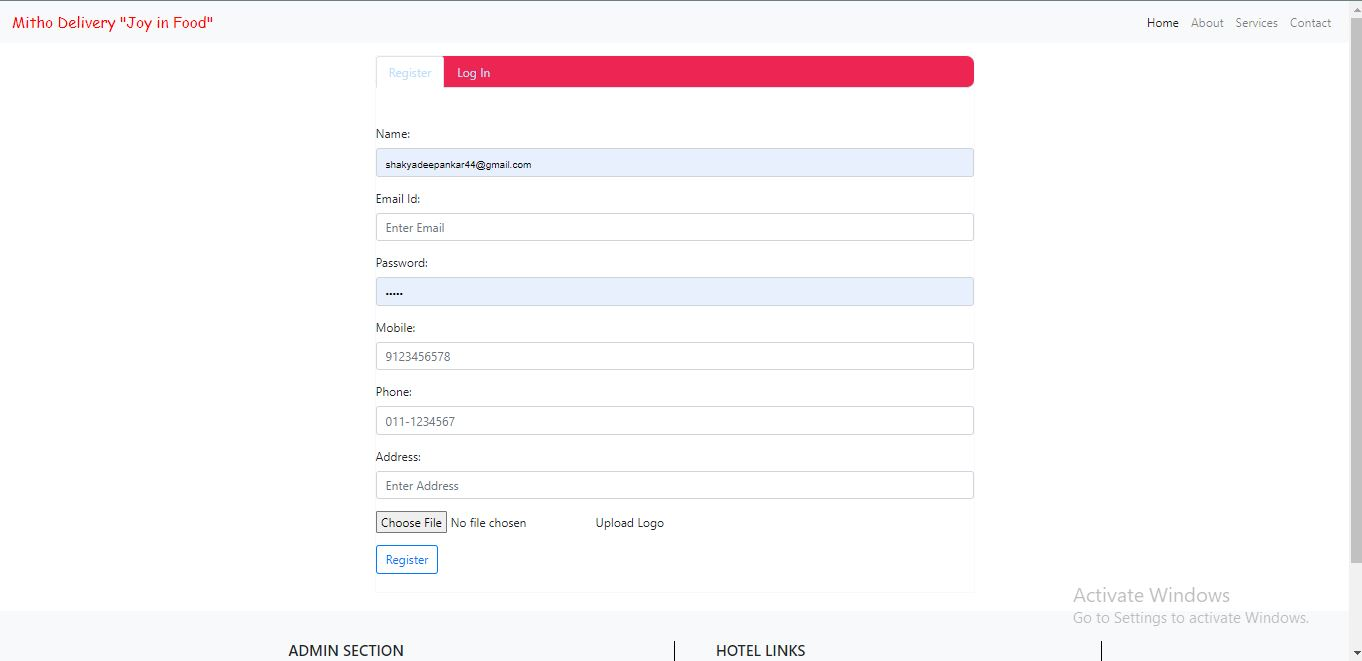
\includegraphics[height=7cm]{img/Graphics/hotel sign up.JPG}
    \caption{Restuarant Signup}
\end{figure}

\newpage
\subsection{Manage Product}
Managing products on a food ordering website involves the process of adding, editing, and organizing menu items that customers can order.
\begin{figure}[h]
    \centering
    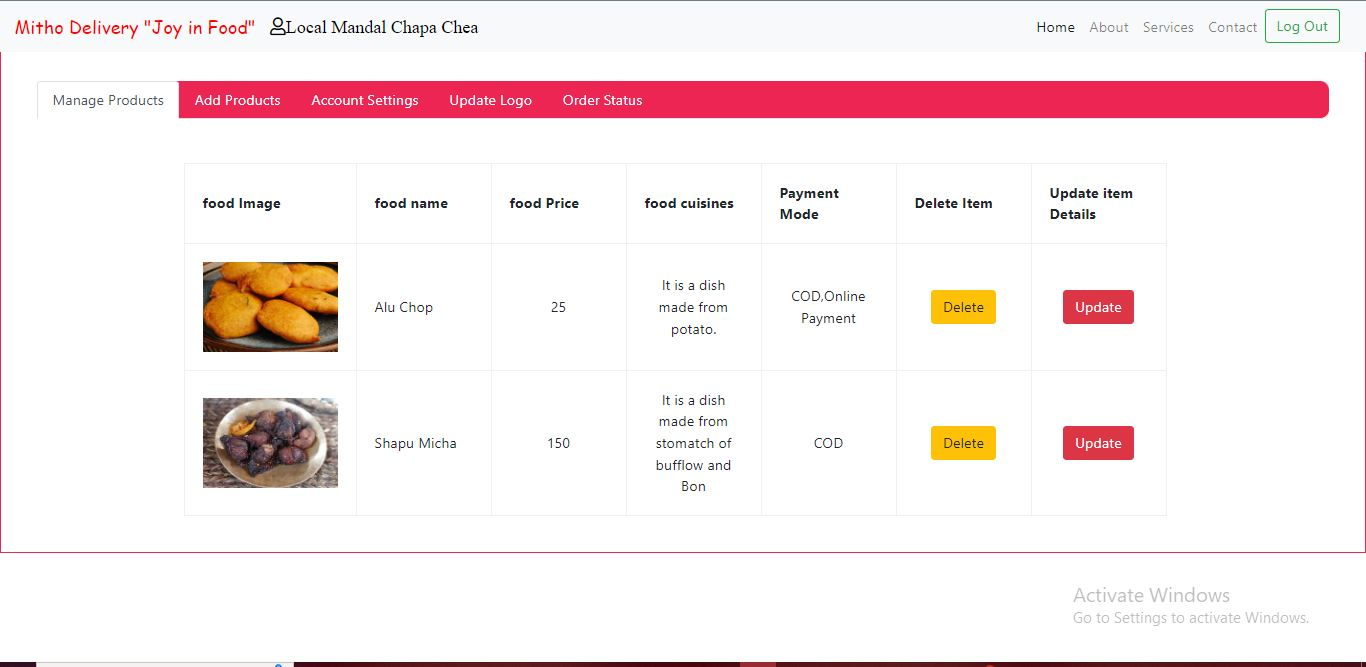
\includegraphics[height=7cm]{img/Graphics/hotel manage product.JPG}
    \caption{Manage Product}
\end{figure}

\subsection{Add Product}
Add Product where Restuarants can add their product here .
\begin{figure}[h]
    \centering
    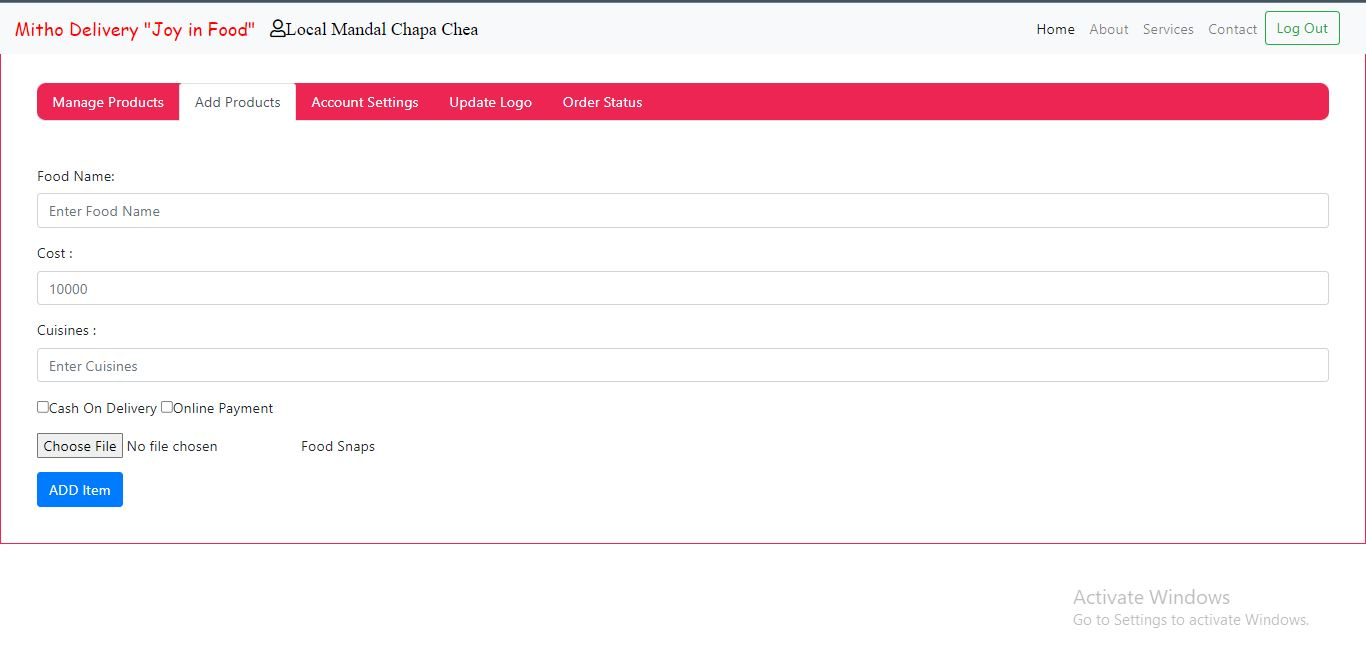
\includegraphics[height=7cm]{img/Graphics/hotel add product.JPG}
    \caption{Add Product}
\end{figure}

\newpage
\subsection{Account Settings}
Account settings on a food ordering website are a crucial feature that allows users to personalize their experience and manage their online profiles.  
\begin{figure}[h]
    \centering
    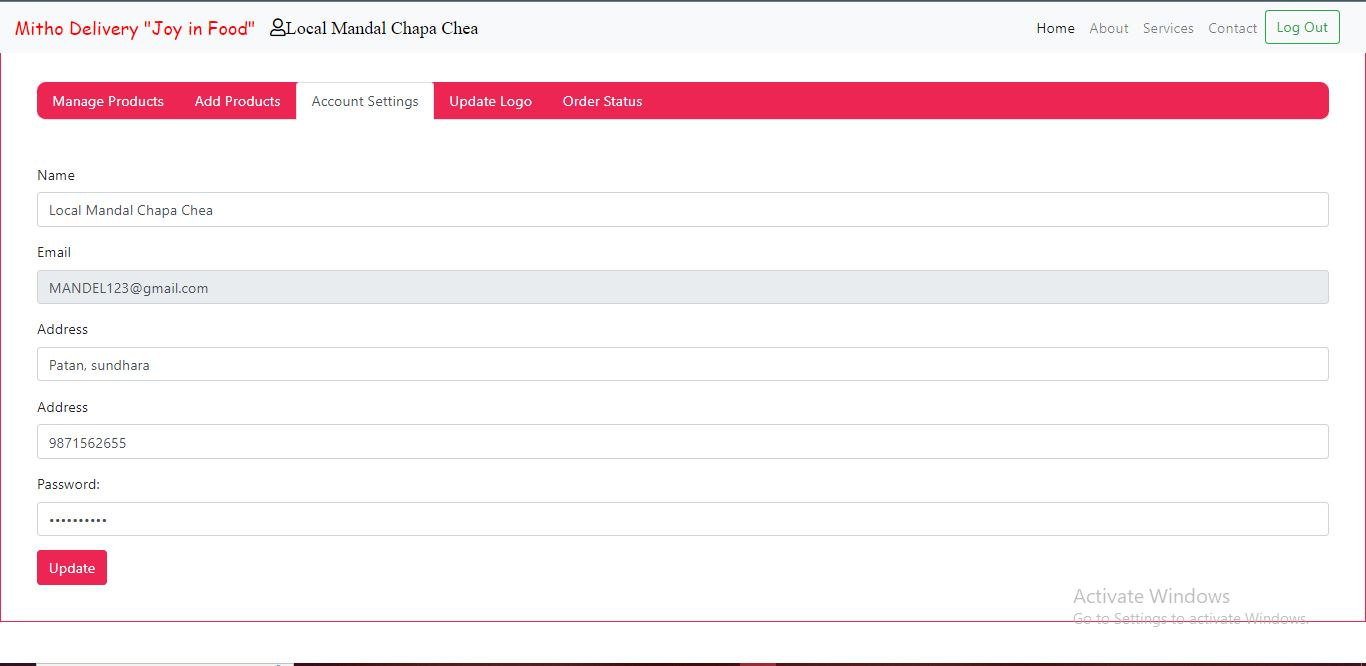
\includegraphics[height=7cm]{img/Graphics/hotel manage account.JPG}
    \caption{Account Settings}
\end{figure}

\subsection{Update Logo}
An update to a website's logo involves changing the visual representation or symbol that identifies the website or brand. This can be done for various reasons, such as rebranding, modernization, or a desire for a fresh look.
\begin{figure}[h]
    \centering
    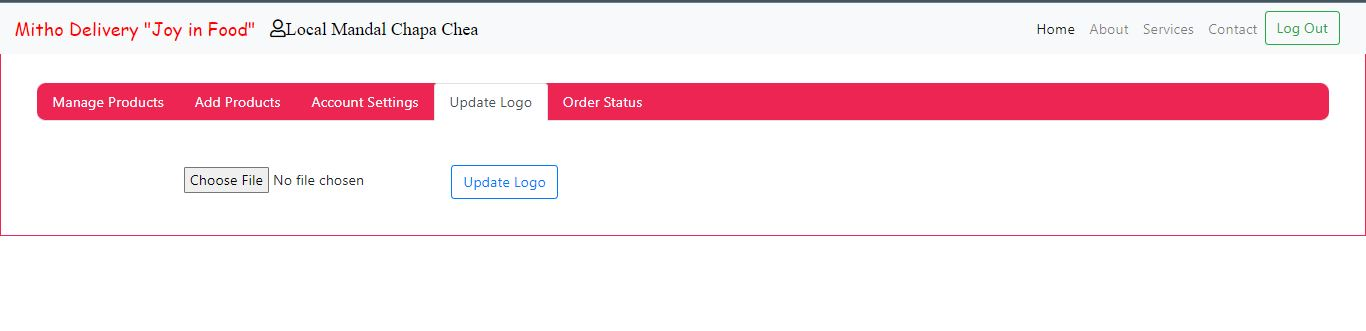
\includegraphics[height=4cm]{img/Graphics/hotel manage logo.JPG}
    \caption{Update Logo}
\end{figure}

\newpage
\subsection{Order Status}
An "Order Status" page on a website is a feature that allows customers and restaurants to monitor the progress of their orders. It typically provides real-time updates on the status of orders, from the moment they are placed to their final delivery
\begin{figure}[h]
    \centering
    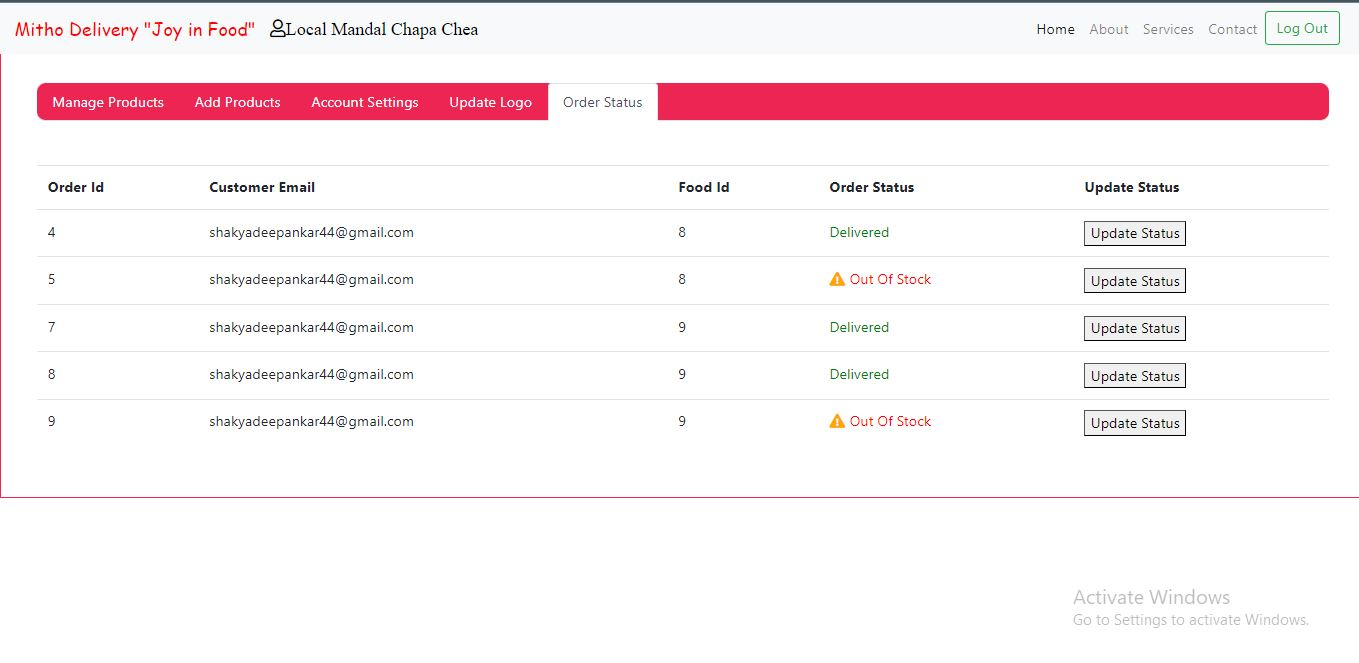
\includegraphics[height=7cm]{img/Graphics/hotel order status.JPG}
    \caption{Order Status}
\end{figure}

\subsection{Manage food}
Managing food on a website from the admin side involves tasks like adding, organizing, and updating food items and categories, setting prices and discounts, controlling inventory, uploading images and descriptions, and overseeing orders.
\begin{figure}[h]
    \centering
    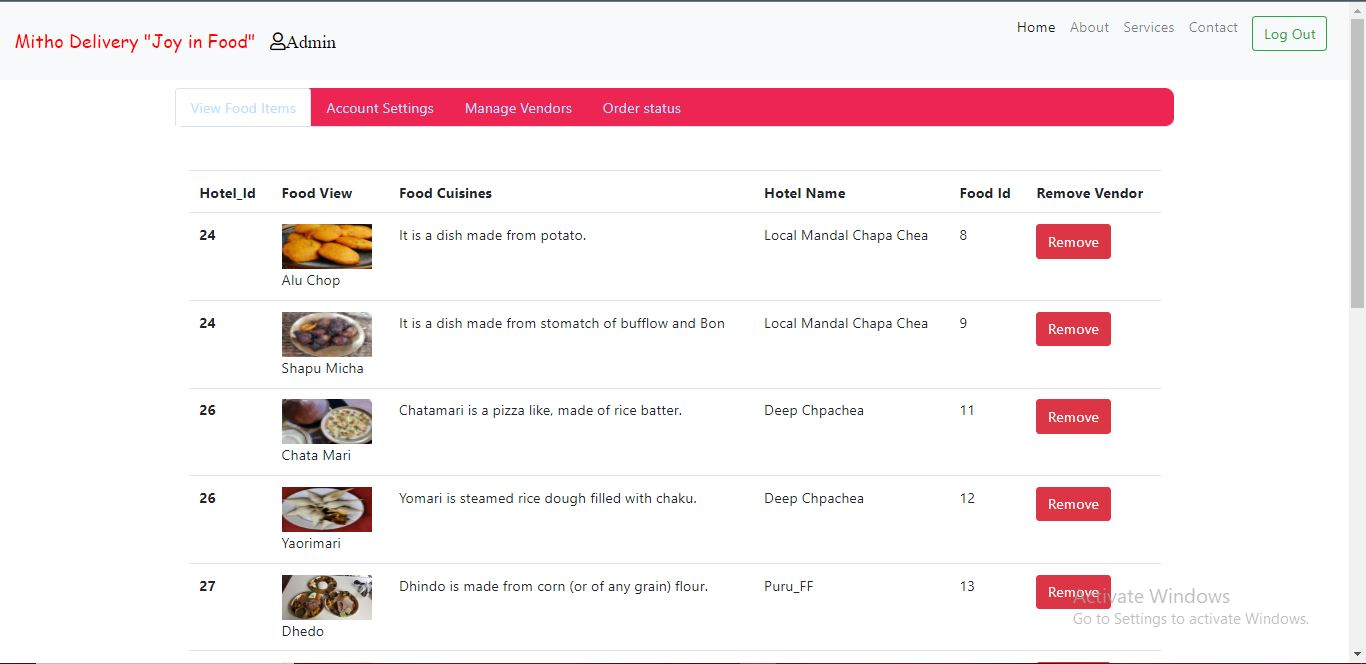
\includegraphics[height=7cm]{img/Graphics/admine manage food.JPG}
    \caption{Manage food}
\end{figure}

\newpage
\subsection{Manage Vendors}
Managing a restaurant from the admin side of a website involves tasks like updating the menu with prices and descriptions, organizing items, and handling online orders and handle restaurant details.
\begin{figure}[h]
    \centering
    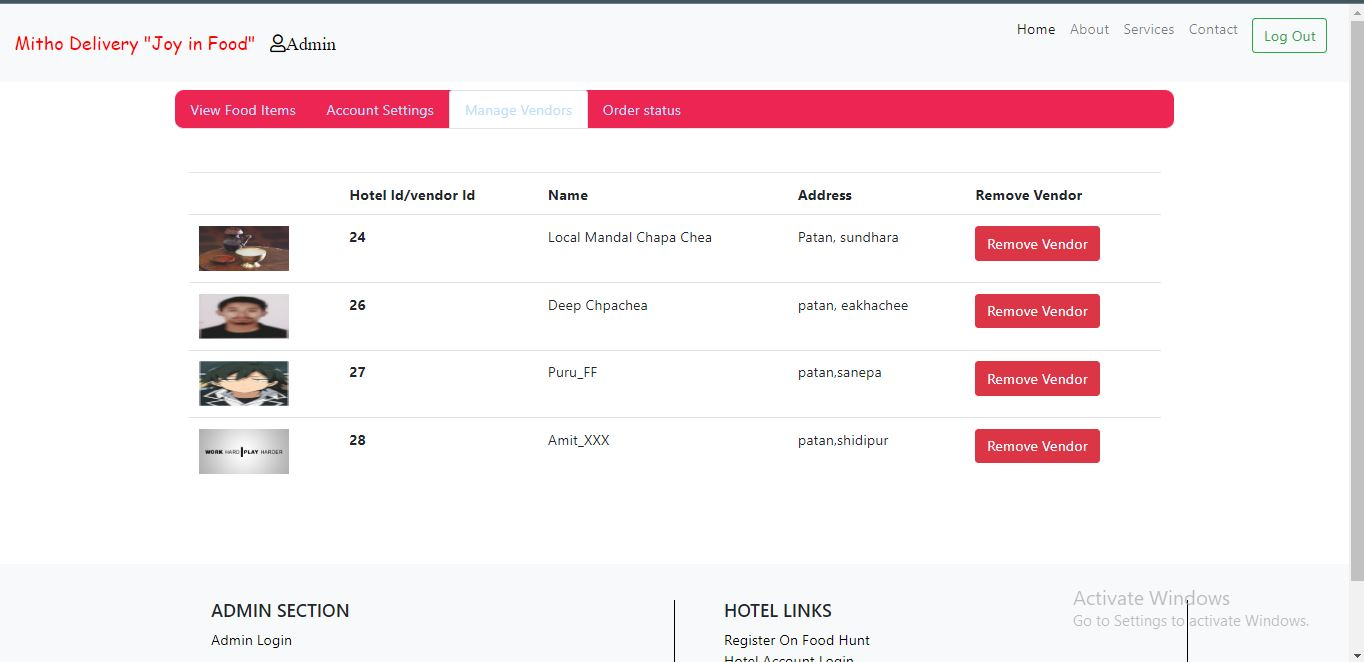
\includegraphics[height=7cm]{img/Graphics/hotel manage vendor (1).JPG}
    \caption{Manage Vendors}
\end{figure}

\subsection{Manage Account}
Managing user accounts of a website involves tasks like creating and maintaining user profiles, controlling access permissions, handling password management, updating user data, monitoring activity, suspending or deactivating accounts when necessary, and ensuring data cleanliness.
\begin{figure}[h]
    \centering
    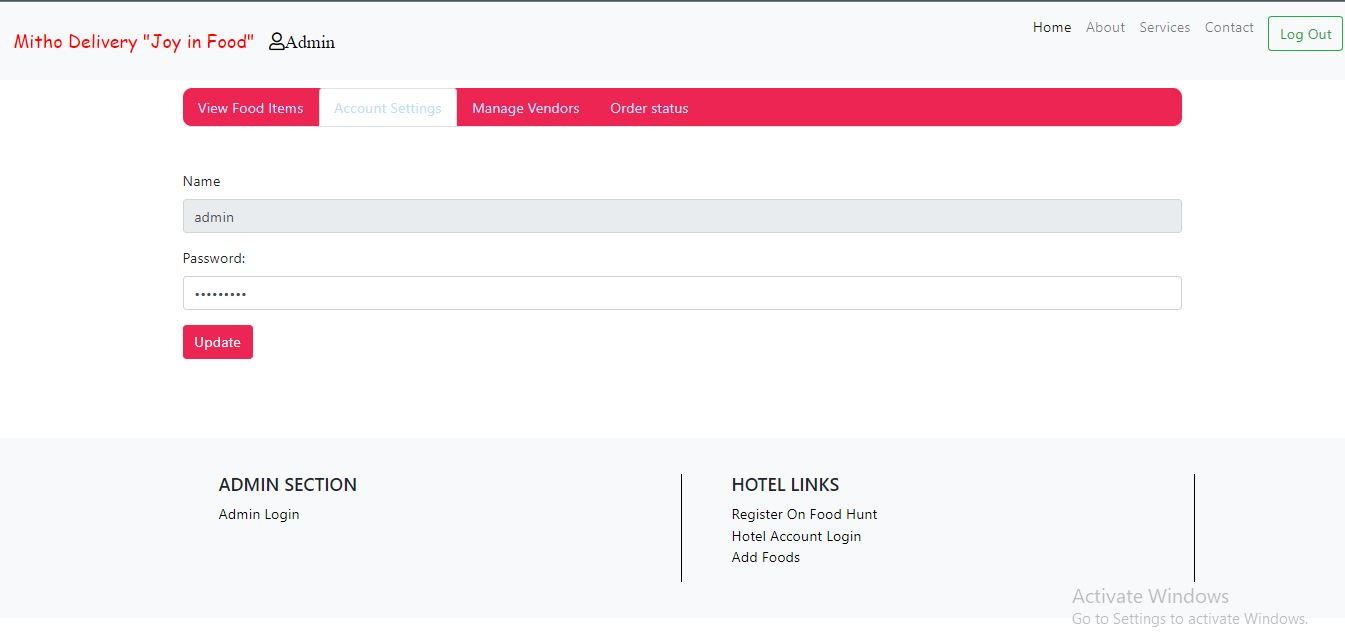
\includegraphics[height=7cm]{img/Graphics/admin manage account.JPG}
    \caption{Manage Account}
\end{figure}


*\subsection*{Database}
A database is a critical component that stores and manages the data needed to power the website's functionality and provide dynamic content to users. Websites often rely on databases to store various types of information, such as user profiles, content, product listings, comments, and more.

\subsection{Admin Database}
Here is an admin database, short for administrative database, is a centralized repository of information used to manage and oversee various aspects of an website's operations.
\begin{figure}[h]
    \centering
    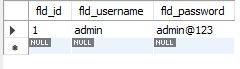
\includegraphics[height=4cm]{img/Graphics/adminDB.JPG}
    \caption{Admin Database}
\end{figure}

\subsection{Customer Database}
Here,customer database is a structured collection of information about an website's customers or clients. It serves as a valuable resource for businesses to manage and analyze customer-related data.
\begin{figure}[h]
    \centering
    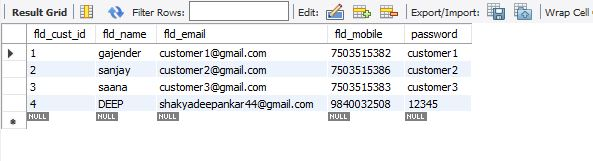
\includegraphics[height=4cm]{img/Graphics/costumerDB.JPG}
    \caption{Customer Database}
\end{figure}

\newpage
\subsection{Vendor Database}
A restaurant database is a structured collection of digital information that stores and manages data related to restaurants, their menus, customer reviews, staff information, and various other aspects of the restaurant industry. 
\begin{figure}[h]
    \centering
    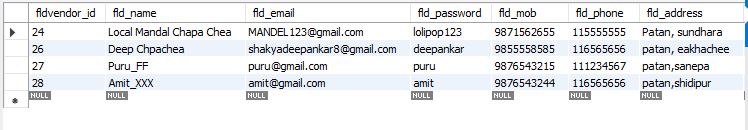
\includegraphics[width=15cm, height=5cm]{img/Graphics/vendorDB.JPG}
    \caption{Vendor Database}
\end{figure}

\subsection{Food Database}
Here, an food database is a comprehensive collection of information about various foods, their nutritional content, and other relevant details.
\begin{figure}[h]
    \centering
    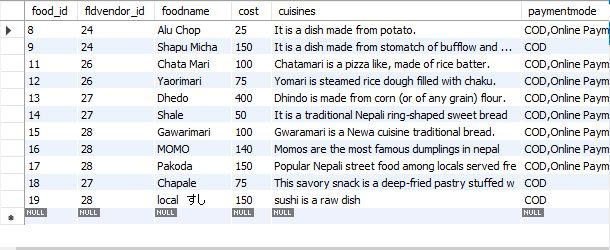
\includegraphics[height=6cm]{img/Graphics/foodDB.JPG}
    \caption{Food Database}
\end{figure}

\newpage
\subsection{Order Database}
Here is an order database that is a structured repository of information that records and manages orders placed by customers or clients. 
\begin{figure}[h]
    \centering
    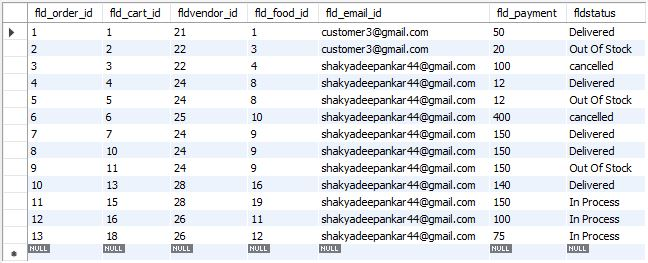
\includegraphics[height=6cm]{img/Graphics/orderDB.JPG}
    \caption{Order Database}
\end{figure}

\subsection{Cart Database}
A cart database is a fundamental component of e-commerce websites and applications. It serves as a digital storehouse for temporarily storing the items a shopper intends to purchase before completing the checkout process. 
\begin{figure}[h]
    \centering
    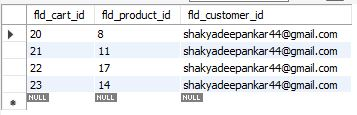
\includegraphics[width=15cm, height=5cm]{img/Graphics/cartDB.JPG}
    \caption{Cart Database}
\end{figure}

\newpage
\subsection{Message Database}
A message database in a food ordering website is a crucial component that facilitates communication between users, restaurants, and the platform itself
\begin{figure}[h]
    \centering
    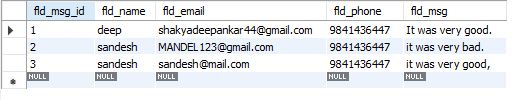
\includegraphics[width=15cm, height=4cm]{img/Graphics/messageDB.JPG}
    \caption{Message Database}
\end{figure}

\section{Conclusion}
In summary, "Mitho Delivery: Joy in Food" is a project aimed at revolutionizing the online food delivery industry by addressing common challenges and providing a user-friendly platform for both customers and restaurants. This project seeks to enhance the convenience and satisfaction of customers while supporting small food businesses and promoting local culinary diversity.
As we embark on this journey, we are committed to overcoming challenges and delivering an exceptional experience to our users, ultimately contributing to the growth of local food businesses and the convenience of customers across Nepal.

\newpage
\section{Future Recommendations}
Here are some future Recommendation for our Website:
\begin{enumerate}
\item {Email Verification with OTP:} Implement a robust email verification system with one-time passwords (OTP). This will enhance security and ensure that users' email addresses are valid, reducing the likelihood of fake accounts and enhancing trust in the platform.

\item {Online Payment with Digital Slips:} Integrate multiple secure online payment options, such as credit/debit cards, digital wallets, and UPI (Unified Payments Interface). Additionally, provide digital payment slips that users can easily access and reference for their orders, improving transparency in financial transactions.

\item {Real-Time Location Tracking:} Enhance the user experience by implementing real-time location tracking for orders. Allow customers to track their delivery in real-time on a map, providing accurate ETAs (Estimated Time of Arrival) and reducing anxiety associated with waiting for food.

\item {Review and Comments System:} Develop a comprehensive review and comments system that encourages user feedback. Allow customers to rate their orders and leave detailed comments. This not only provides valuable feedback for restaurants but also helps other users make informed decisions based on genuine experiences.

\item {Recommendation AI:} Utilize artificial intelligence and machine learning algorithms to provide personalized food recommendations. Consider the user's location, previous orders, and ratings to suggest restaurants and dishes that align with their preferences. This can significantly enhance the user experience and drive increased engagement.
\end{enumerate}

\newpage
\chapter{DISCUSSION AND ANALYSIS}
This project report comprehensively evaluates the performance of a food delivery website, focusing on the comparison between initial predictions and actual outcomes during implementation. Projections of gradual user engagement growth, order increases, and revenue generation encountered deviations due to complex user behavior, external influences like competitors and economic shifts, and technical challenges. These factors collectively led to disparities in the expected and observed results.
Comparative analysis with established food delivery services revealed commendable performance metrics, including comparable order volume, favorable user reviews, and distinctive features like personalized recommendations and optimized delivery logistics. Despite these achievements, challenges emerged, such as slower user acquisition and technical glitches affecting early user satisfaction.

This project's journey in developing a competitive food delivery website highlights the significance of addressing intricate user behavior, external dynamics, and technical issues. A commitment to continual improvement, including rectifying technical shortcomings and embracing machine learning for enhanced user experiences, underscores the project's ongoing evolution in the dynamic landscape of food delivery websites.

